\chapter{Gestione delle reti}
Una rete di comunicazione viene concepita, implementata e gestita con uno o più \textit{scopi} come, ad esempio, una \textit{rete telefonica}, per comunicazioni vocali tra individui, una rete \textit{internet}, per il trasferimento e la condivisione di dati eterogenei, etc. Vi è molta differenza tra gli \textit{obiettivi} con cui una rete viene concepita (protocolli, standard, etc.) e quelli con cui questa viene \textit{gestita} dagli operatori; sicuramente il \textit{tempo} ed il \textit{business} sono due fattori determinanti.\\
Con il termine \textbf{management} si intendono tutte le operazioni che assicurano l'effettivo ed efficiente utilizzo di un sistema di comunicazioni e delle sue risorse in accordo con gli obiettivi aziendali. Si noti comunque che questa definizione è generica, può essere applicata anche a sistemi diversi da quelli di telecomunicazioni e gli \textit{obiettivi aziendali} possono essere correlati o meno con le telecomunicazioni.
\begin{figure}[htbp]
	\centering
	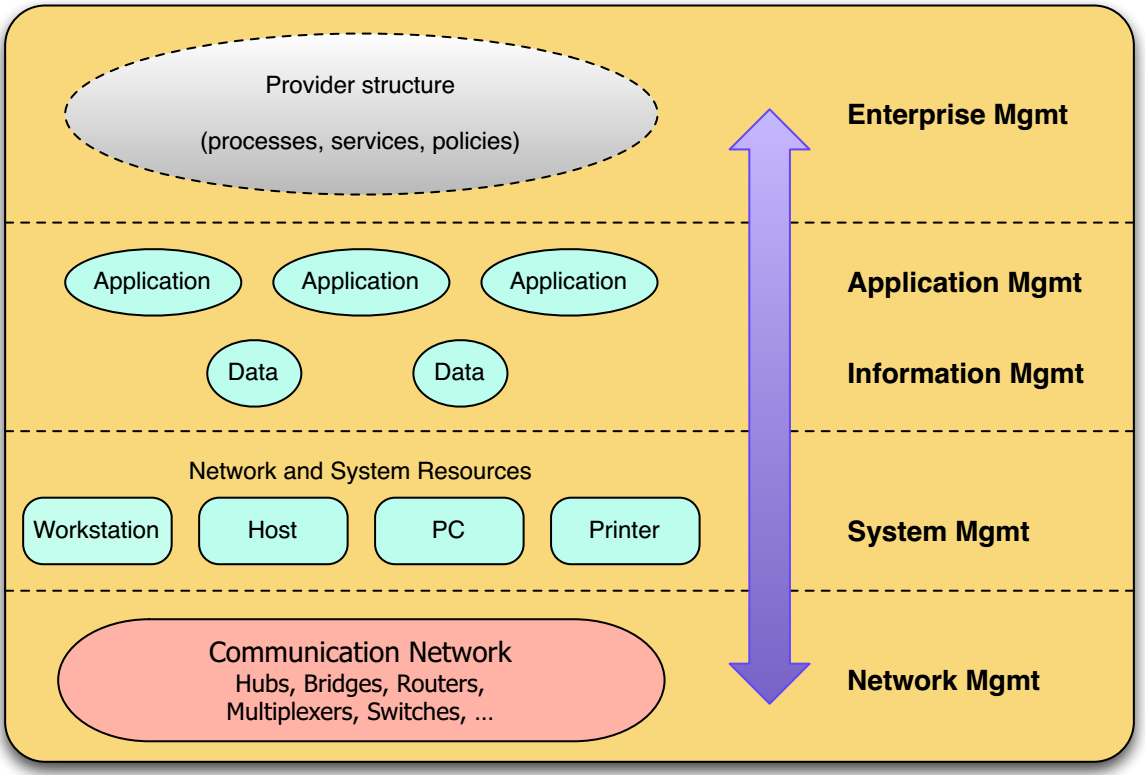
\includegraphics[scale = 0.4]{images/management_levels}
	\caption{Livelli di management.}
	\label{img:management_levels}
\end{figure}\\
In Figura \ref*{img:management_levels} sono rappresentati i livelli del management, iniziamo a descriverli dal basso. Il \textit{network management} mira ad occuparsi della gestione delle risorse di comunicazione, come ad esempio switch, router, linee, protocolli, etc., e dei servizi da essi offerti. Il \textit{system management} si occupa della gestione delle risorse dei sistemi finali e dei sistemi connessi alla rete (terminali, telefoni, servers, etc.). L'\textit{application management} tende ad occuparsi della gestione delle applicazioni distribuite (o meno) e dei servizi offerti in modo distribuito come e-mail e file sharing clusterizzato. Nell'\textit{enterprise management} o \textit{management integrato}, infine, tutti i livelli di management concorrono allo stesso scopo.
\begin{figure}[htbp]
	\centering
	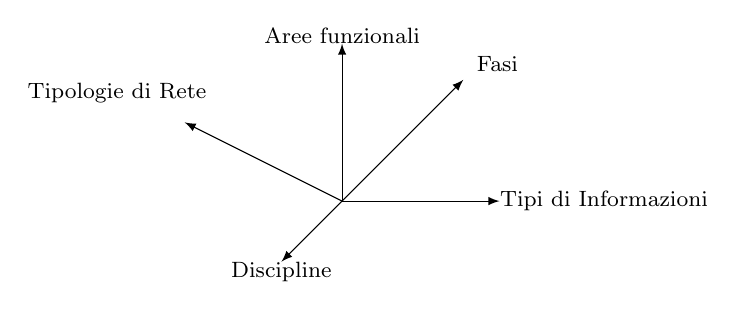
\begin{tikzpicture}
		\tikzset{mynode/.style={font=\footnotesize,inner sep=0pt,text=black}}
		%Begin plot
		\draw[-latex] (0,0,0) -- (2,0,0)node[mynode,anchor=west]{Tipi di Informazioni};
		\draw[-latex] (0,0,0) -- (0,2,0)node[mynode,anchor=south]{Aree funzionali};
		\draw[-latex] (0,0,0) -- (0,0,2)node[mynode,anchor=north]{Discipline};
		\draw[-latex] (0,0,0) -- (-2,1,0)node[mynode,anchor=north west,xshift=-2cm,yshift=0.5cm]{Tipologie di Rete};
		\draw[-latex] (0,0,0) -- (0,0,-4)node[mynode,anchor=north east,xshift=0.7cm,yshift=0.3cm]{Fasi};	
	\end{tikzpicture}
	\caption{Tipi di management.}
	\label{img:management_types}
\end{figure}\\
Come è possibile osservare dalla Figura \ref{img:management_types} vi sono vari tipi di management. Le \textit{aree funzionali} comprendono tutto ciò che riguarda configuration, performance, fault, security, accounting. Le \textit{fasi}, invece, planning, installation, operation, change, dismissing. Le \textit{tipologie di rete} comprendono internet, VPN, corporate, WAN, LAN, etc. Non esiste dunque un solo sistema di management e quindi non esiste una sola soluzione per il management, contando il fatto che non abbiamo parlato di organizzazione, fattori economici e legali, etc. Sostanzialmente l'idea fondamentale è quella di \textit{utilizzare concetti e formati standard per permettere l'interscambio di informazioni tra i fari livelli di management e tra le entità che lo compongono} (integrated management).

\noindent Vediamo adesso la \textit{management architecture}, ossia l'insieme degli standard relativi al management. Questa è suddivisa in:
\begin{itemize}
	\item \textbf{Information model}. Descrive il sistema sintattico e semantico per la rappresentazione delle risorse e delle informazioni in maniera orientata al management e indipendente dal venditore.
	\item \textbf{Communication model}. Descrive il sistema di accesso agli oggetti gestiti ed i protocolli di management.
	\item \textbf{Function model}. Organizza il sistema di management in sotto-task più gestibili e definisce funzioni di management generiche.
	\item \textbf{Organization model}. Definisce ruoli, modelli di cooperazione e domini di competenza.
\end{itemize}
L'unione dell'information e del communication model rappresenta gli \textquotedblleft elementi" hardware e software abbastanza comprensibili da un ingegnere, mentre l'unione di function ed organization model rappresenta gli \textquotedblleft elementi" organizzativi imprescindibili che coinvolgono persone e non macchine. Tutta questa architettura concorre a definire la \textbf{management platform}, che può (a volte) essere composta da elementi semplici, utilizzabili anche singolarmente (e.g. ping).

Per chi e perché viene attuato il management? In sostanza:
\begin{itemize}
	\item L'\textit{utente} finale è interessato ad avere un sistema affidabile, flessibile, sicuro, efficace, poco costoso, etc. e non è interessato a come viene realizzato. Tuttavia, le esigenze dell'utente sono alla base del management.
	\item L'\textit{azienda} vuole trarre profitti e anch'essa non è interessata a come un sistema viene realizzata. Tuttavia, anche le esigenze dell'azienda sono alla base del management.
\end{itemize}
Gli obiettivi del management devono dunque essere quelli di offrire all'utente il \textquotedblleft prodotto" (QoS, banda, whatever) richiesto e di gestire al meglio le risorse a disposizione evitando gli sprechi.